\documentclass[%
crop,%
tikz,%
convert={outext=.svg,command=\unexpanded{pdf2svg \infile\space../_static/\outfile}},%
multi=false%
]{standalone}%
\usepackage[utf8]{luainputenc}%
\usepackage[no-math]{fontspec}%
\defaultfontfeatures{%
    Numbers={OldStyle,Proportional},%
    Ligatures=TeX,%
    Extension=.ttf,%
}%
\setmainfont[%
UprightFont=*-Regular,%
ItalicFont=*-Italic,%
BoldFont=*-Bold,%
BoldItalicFont=*-BoldItalic,%
]{Raleway}%
\setsansfont[%
UprightFont=*-Regular,%
ItalicFont=*-Italic,%
BoldFont=*-Bold,%
BoldItalicFont=*-BoldItalic,%
]{Raleway}%
\usepackage[frenchmath]{mathastext}%
\usepackage{amsmath}%
\usepackage{amssymb}%
\usepackage{mathrsfs}%
\usepackage{mathtools}%
\usepackage{siunitx}%
\usepackage[siunitx]{circuitikz}%
\usetikzlibrary{calc,backgrounds,arrows.meta,patterns}%

\DeclareMathOperator{\sign}{sign}%

% Ensembles
\let\C\relax
\newcommand{\R}{\ensuremath{\mathbb{R}}} % Réel
\newcommand{\N}{\ensuremath{\mathbb{N}}} % Entiers naturels
% \newcommand{\C}{\ensuremath{\mathbb{C}}} % Complexes
\newcommand{\B}{\ensuremath{\mathscr{B}}} % Bus électriques
\newcommand{\Ch}{\ensuremath{\mathscr{C}}} % Charges
\renewcommand{\L}{\ensuremath{\mathscr{L}}} % Lignes
\renewcommand{\P}{\ensuremath{\mathscr{P}}} % Phases

% Phases
\newcommand{\arm}{\ensuremath{\mathrm{a}}}%
\newcommand{\brm}{\ensuremath{\mathrm{b}}}%
\newcommand{\crm}{\ensuremath{\mathrm{c}}}%
\newcommand{\nrm}{\ensuremath{\mathrm{n}}}%
\newcommand{\trm}{\ensuremath{\mathrm{t}}}%
\newcommand{\grm}{\ensuremath{\mathrm{g}}}%
\newcommand{\abrm}{\ensuremath{\mathrm{ab}}}%
\newcommand{\bcrm}{\ensuremath{\mathrm{bc}}}%
\newcommand{\carm}{\ensuremath{\mathrm{ca}}}%
\newcommand{\anrm}{\ensuremath{\mathrm{an}}}%
\newcommand{\bnrm}{\ensuremath{\mathrm{bn}}}%
\newcommand{\cnrm}{\ensuremath{\mathrm{cn}}}%
\newcommand{\atrm}{\ensuremath{\mathrm{at}}}%
\newcommand{\btrm}{\ensuremath{\mathrm{bt}}}%
\newcommand{\ctrm}{\ensuremath{\mathrm{ct}}}%
\newcommand{\ntrm}{\ensuremath{\mathrm{nt}}}%
\newcommand{\agrm}{\ensuremath{\mathrm{ag}}}%
\newcommand{\bgrm}{\ensuremath{\mathrm{bg}}}%
\newcommand{\cgrm}{\ensuremath{\mathrm{cg}}}%
\newcommand{\ngrm}{\ensuremath{\mathrm{ng}}}%
\newcommand{\abcrm}{\ensuremath{\mathrm{abc}}}%
\newcommand{\abcnrm}{\ensuremath{\mathrm{abcn}}}%

% Indices ou exposants
\newcommand{\cons}{\ensuremath{\mathrm{cons.}}}%
\renewcommand{\prod}{\ensuremath{\mathrm{prod.}}}%
\newcommand{\theo}{\ensuremath{\mathrm{th.}}}%
\newcommand{\const}{\ensuremath{\mathrm{const.}}}%

% Variables
\newcommand{\umax}{\ensuremath{U^{\max}}}%
\newcommand{\umaxnorm}{\ensuremath{U^{\max\,\text{norm.}}}}%
\newcommand{\umin}{\ensuremath{U^{\min}}}%
\newcommand{\uminnorm}{\ensuremath{U^{\min\,\text{norm.}}}}%
\newcommand{\unom}{\ensuremath{U^{\text{nom.}}}}%
\newcommand{\unomnorm}{\ensuremath{U^{\text{nom.}\,\text{norm.}}}}%
\newcommand{\uup}{\ensuremath{U^{\text{up}}}}%
\newcommand{\uupnorm}{\ensuremath{U^{\text{up}\,\text{norm.}}}}%
\newcommand{\uupprime}{\ensuremath{U^{\text{up}\,\prime}}}%
\newcommand{\udown}{\ensuremath{U^{\text{down}}}}%
\newcommand{\udownnorm}{\ensuremath{U^{\text{down}\,\text{norm.}}}}%
\newcommand{\udownprime}{\ensuremath{U^{\text{down}\,\prime}}}%
\newcommand{\smax}{\ensuremath{S^{\max}}}%
\newcommand{\pmax}{\ensuremath{P^{\max}}}%
\newcommand{\sproj}{\ensuremath{\underline{S^{\text{proj.}}}}}%
%

\usepackage{pgfplots}%
\pgfplotsset{compat=newest}%
\usepgfplotslibrary{groupplots, colorbrewer}%

\begin{document}
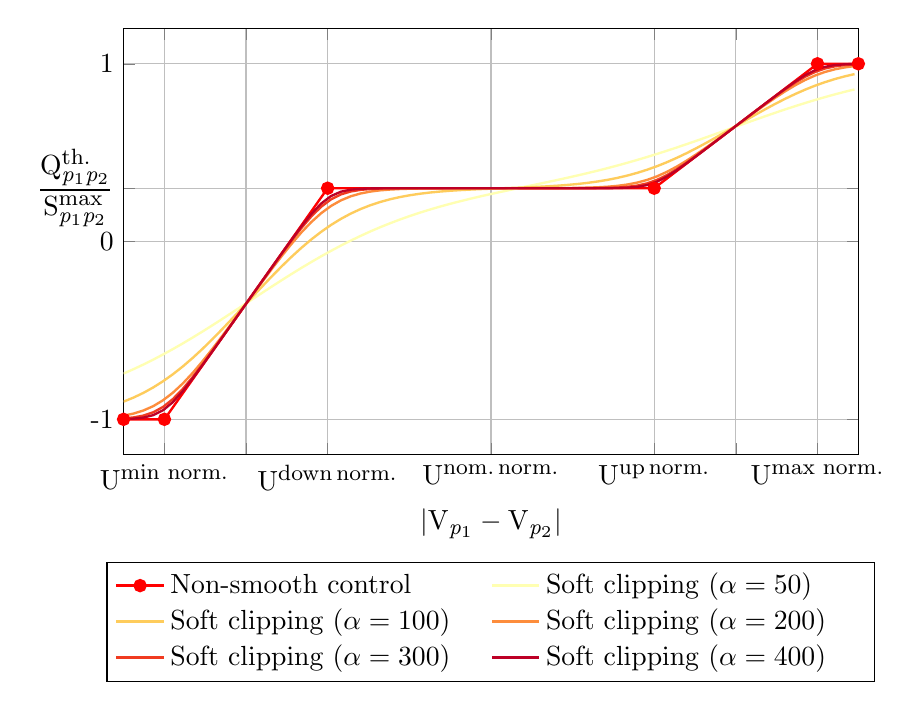
\begin{tikzpicture}[%
    show background rectangle,%
    tight background,%
    background rectangle/.style={fill=white}%
  ]
  %
  % Common parameters
  %
  \pgfmathsetmacro{\umaxvaleur}{250.0}%
  \pgfmathsetmacro{\umaxnormvaleur}{1.0}%
  \pgfmathsetmacro{\uupvaleur}{240.0}%
  \pgfmathsetmacro{\uupnormvaleur}{\uupvaleur/\umaxvaleur}%
  \pgfmathsetmacro{\udownvaleur}{220.0}%
  \pgfmathsetmacro{\udownnormvaleur}{\udownvaleur/\umaxvaleur}%
  \pgfmathsetmacro{\uminvaleur}{210.0}%
  \pgfmathsetmacro{\uminnormvaleur}{\uminvaleur/\umaxvaleur}%
  \pgfmathsetmacro{\unomvaleur}{(\udownvaleur+\uupvaleur)/2.0}%
  \pgfmathsetmacro{\unomnormvaleur}{\unomvaleur/\umaxvaleur}%
  \pgfmathsetmacro{\umidminvaleur}{(\udownvaleur+\uminvaleur)/2.0}%
  \pgfmathsetmacro{\umidminnormvaleur}{\umidminvaleur/\umaxvaleur}%
  \pgfmathsetmacro{\umidmaxvaleur}{(\uupvaleur+\umaxvaleur)/2.0}%
  \pgfmathsetmacro{\umidmaxnormvaleur}{\umidmaxvaleur/\umaxvaleur}%

  \pgfmathsetmacro{\xminvaleur}{\uminvaleur - 2.5}%
  \pgfmathsetmacro{\xminnormvaleur}{\xminvaleur/\umaxvaleur}%
  \pgfmathsetmacro{\xmaxvaleur}{\umaxvaleur + 2.5}%
  \pgfmathsetmacro{\xmaxnormvaleur}{\xmaxvaleur/\umaxvaleur}%

  \pgfmathsetmacro{\yminnormvaleur}{-1}%
  \pgfmathsetmacro{\ymaxnormvaleur}{1}%

  \pgfmathsetmacro{\qthnormvaleur}{0.30}%

  %
  % Style
  %
  \tikzset{lisse/.style={line width=0.3mm, domain=\xminnormvaleur:\xmaxnormvaleur, samples=75,
      mark=none}}%
  \tikzset{non lisse/.style={line width=0.3mm, mark=*}}%

  \begin{axis}
    [%
    height=7cm,%
    width=0.9\textwidth,%
    enlarge y limits,%
    grid=major,%
    xlabel={$|V_{p_1}-V_{p_2}|$},%
    xtick={\uminnormvaleur,\umidminnormvaleur,\udownnormvaleur,\unomnormvaleur,\uupnormvaleur,\umidmaxnormvaleur,\umaxnormvaleur},%
    xticklabels={%
      $\uminnorm$,,$\udownnorm$,$\unomnorm$,$\uupnorm$,,$\umaxnorm$%
    },%
    y tick label style={%
      /pgf/number format/.cd,%
      set thousands separator={},%
      fixed,%
      fixed zerofill,%
      precision=1,%
      use comma%
    },%
    ytick={\yminnormvaleur,0,\qthnormvaleur,\ymaxnormvaleur},%
    yticklabels={-1,0,$\dfrac{Q^{\theo}_{p_1p_2}}{\smax_{p_1p_2}}$,1},%
    xmin=\xminnormvaleur,%
    xmax=\xmaxnormvaleur,%
    ymin=\yminnormvaleur,%
    ymax=\ymaxnormvaleur,%
    legend columns=2,%
    legend style={%
      at={(0.5,-0.25)},%
      anchor=north,%
      nodes={text width=4cm}%
    },%
    cycle list/YlOrRd-5,%
    cycle list name=YlOrRd-5%
    ]%%%%%%% initialize YlOrRd-5%

    % Fonction linéaire par morceaux
    \addplot[non lisse, red] coordinates {%
        (\xminnormvaleur,-1)%
        (\uminnormvaleur,-1)%
        (\udownnormvaleur,\qthnormvaleur)%
        (\uupnormvaleur,\qthnormvaleur)%
        (\umaxnormvaleur,1)%
        (\xmaxnormvaleur,1)%
      };%
    \addlegendentry{Non-smooth control};%

    % Soft clipping functions
    \pgfplotsset{cycle list shift=-1}% Reset cycle to 0
    \foreach \alphavaleur in {50,100,200,300,400} {%
        \addplot+[lisse] expression {%
            \qthnormvaleur + ( 1.0/(\alphavaleur*(\uminnormvaleur-\udownnormvaleur)) *
            ln((1+exp(\alphavaleur*(x-\udownnormvaleur)))/(1+exp(\alphavaleur*(x-\uminnormvaleur))))-1.0
            )*(1+\qthnormvaleur) + ( 1.0/(\alphavaleur*(\umaxnormvaleur-\uupnormvaleur)) *
            ln((1+exp(\alphavaleur*(x-\uupnormvaleur)))/(1+exp(\alphavaleur*(x-\umaxnormvaleur))))
            )*(1-\qthnormvaleur) };%
        \addlegendentryexpanded{Soft clipping ($\alpha=\num{\alphavaleur}$)};%
      };%
  \end{axis}
\end{tikzpicture}
\end{document}
% Local Variables:
% mode: latex
% TeX-engine: luatex
% TeX-source-correlate-method-active: synctex
% ispell-local-dictionary: "british"
% coding: utf-8
% LaTeX-indent-level: 2
% fill-column: 120
% End:
